\section{Versuchsauswertung}

\subsection{Solarstrahlung} 

\subsubsection{Aufnahme der Messdaten}

Der Schattenring des CM11 Pyranometers zur Messung der Diffusstrahlung wurde nach Tabelle 5 des Praktikumsskriptes ausgerichtet. Die Ausrichtung der Messtafel mit den übrigen Sensoren Richtung Sonne konnte nur geschätzt werden, da der Himmel zum Zeitpunkt der Messung bedeckt war. Für die weitere Auswertung wird daher ein bereitgestellter Datensatz (vgl. Abbildung \ref{fig:radiation}) verwendet.

\begin{figure}[H]
	\centering
	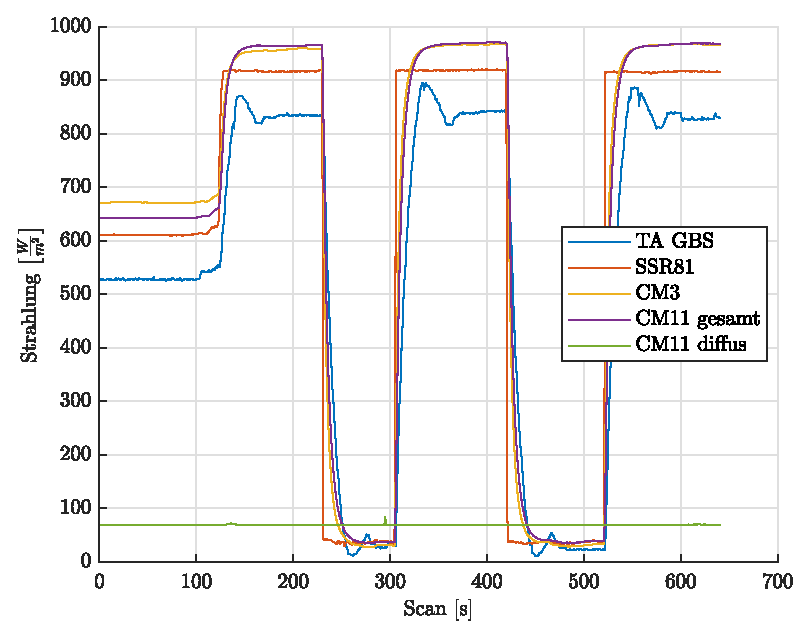
\includegraphics[width=\textwidth]{../DATA/Messreihe_Strahlung.eps}
	\caption[Messreihe zur Bestimmung der Solarstrahlung]{Messreihe zur Bestimmung der Solarstrahlung}
	\label{fig:radiation}
\end{figure}
Zum Vergleich der Messwerte wurden der Mittelwert und die Standardabweichung der einzelnen Sensoren über den stationären Messbereich zwischen Sekunde 170 und Sekunde 220 gebildet. Tabelle 1 zeigt die bestimmten Werte. Die angegeben Strahlungswerte beziehen sich auf die Globalstrahlung. Das mit einem Schattenring ausgestattete CM11 Pyranometer misst hingegen nur die Diffusstrahlung. Die Direktstrahlung kann mittels  Gleichung 1 aus den beiden CM11 Pyranometern berechnet werden.

\begin{table}[H]
	\centering
	\caption{Gemessene Strahlungsstärken der verschiedenen Sensoren.}
\begin{tabular}{l S[separate-uncertainty,table-parse-only,table-figures-uncertainty = 1]}
	\textbf{Sensor} & \textbf{Strahlung [E] = $\frac{W}{m^2}$}\\
	\hline
		TA GBS & 833,6(21)\\
		SSR81 & 916,5(7)\\
		CM3 & 957,8(17)\\
		CM11 & 964,5(4)\\
		CM11 (diffus) & 68,7(2)
%	TA GBS & 833,6252 $\pm$2,1081\\
%	SSR81 & 916,4836 $\pm$0,6581\\
%	CM3 & 957,7781 $\pm$1,7451\\
%	CM11 & 964,5125 $\pm$0,4149\\
%	CM11 (diffus) & 68,6927 $\pm$0,1916
\end{tabular} 

	\label{tab:radiation}
\end{table}

\begin{equation}
	\label{eq:Edir}
	E_{\text{dir}}=E_{\text{global}}-E_{\text{diffus}}=\SI{964.5125}{\watt\per\square\meter}-\SI{68.692}{\watt\per\square\meter} = \SI{895.8205}{\watt\per\square\meter}
\end{equation}

Aus dem Datensatz geht hervor, dass die Halbleitersensoren verglichen mit den Pyranometern eine geringere Strahlung messen. Der induzierte Photoeffekt ist bei Halbleitersensoren abhängig von der Wellenlänge. Aufgrund dieser Verluste wird ein niedrigere Ausgangsspannung am Messwiderstand gemessen. Für eine genauere Messung müsste der Sensor anhand einer definierten Strahlungsleistung (Bsp. Sonnensimulator) kalibriert werden. Weiterhin sind die verwendeten Halbleitersensoren nach keinem Standard klassifiziert, sodass keine nähere Aussage über die messgenauigkeit getroffen werden kann. Thermosäulen liefern präzisere Messwerte, da sie ein Thermisches Messverfahren nutzen und Verluste durch den Glasdom gemindert werden. Die verwendeten CM11 Pyranometer sind nach dem Secondary Standard klassifiziert und sollten daher im Rahmen des Versuchs als Referenz betrachtet werden.


\subsubsection{Bestimmung des Ansprechverhaltens}
Wie im vorherigen Teil der Auswertung wurden bereitgestellte Daten verwendet. Die Messreihe ist in Abbildung \ref{fig:response} gezeigt.Bei Scannr. 89 wurde die Abdeckung entfernt, bei Scannr. 132 haben alle Sensoren den Zielwert erreicht.
\begin{figure}[H]
	\centering
	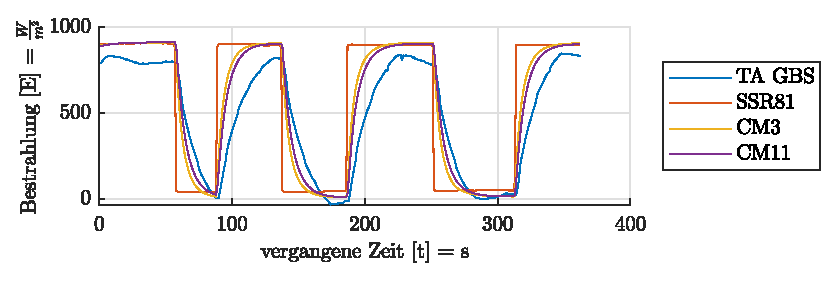
\includegraphics[width=\textwidth]{../DATA/Messreihe_Ansprechzeit.eps}
	\caption[Messreihe zur Bestimmung des Ansprechverhaltens.]{Messreihe zur Bestimmung des Ansprechverhaltens.}
	\label{fig:response}
\end{figure}

\begin{table}[H]
\centering
\caption{Ausgabewerte der Sensoren zur Bestimmung des Ansprechverhaltens.}
	\begin{tabular}{c c c c c}
		\label{tab:response}
		
		\textbf{Sensor} & \textbf{Minimum} $\frac{W}{m^2}$ & \textbf{Maximum} $\frac{W}{m^2}$& \textbf{95\% Threshold} $\frac{W}{m^2}$ & \textbf{Ansprechzeit} s\\
		\hline
		TA GBS & 8,8 & 824,1 & 782,9 & 36 \\
		SSR 81 & 43,5 & 898,7 & 853,8 & 1 \\
		CM 3 & 15,1 & 908,0 & 862,4 & 18 \\
		CM11 & 25,8 & 903,9 & 858,7 & 22 \\
	\end{tabular}
\end{table}
Den Erwartungen entsprechend reagiert der SSR 81 Halbleiter direkt auf die Verschattung, während die Pyranometer eine Latenz aufweisen. Der TA GBS verzögert für einen Halbleiter ungewöhnlich lang.

\subsection{Luftfeuchtemessung}
Zunächst wurden die Umgebungstemperatur und die Ausgangsspannung des Feuchtesensors ermittelt. Zur Bestimmung der relativen Feuchte wurde eine Kalibriergerade anhand zweier Messpunkte angefertigt. Hierzu wurde die Ausgangsspannung des Sensors zunächst über einer NaCl-Lösung, anschließend über einer LiCl-Lösung gemessen. Der Messverlauf ist in Abbildung \ref{fig:cal} aufgetragen. Es wurden jeweils die letzten 100 Scans zur Bestimmung der Ausgangsspannung gemittelt. Bei der vorliegenden Umgebungstemperatur von ca. \SI{24}{\celsius} entspricht die relative Luftfeuchte über NaCl 75\,\%, über LiCl 12\,\%. Die nachfolgende Tabelle zeigt die ermittelten Größen.
\begin{table}[H]
	\centering
	\caption{Ermittelte Größen zur Bestimmung der relativen Luftfeuchte.}
	\begin{tabular}{lS[separate-uncertainty,table-parse-only,table-figures-uncertainty = 1]c}
		\label{tab:amb}
		
		\textbf{Messgröße} & \textbf{Mittelwerte} & \textbf{Lit. rel. Feuchte}\\
		\hline
		Umgebungstemperatur & 24,10(4) \si{\celsius} &\\
		Umgebungsluftfeuchte & 5,979(28) \si{\volt} & \\
		LiCl & 1,330(5) \si{\volt} & 12\,\%\\
		NaCl & 7,243(6) \si{\volt} & 75\,\%
	\end{tabular}
\end{table}

\begin{figure}[H]
	\centering
	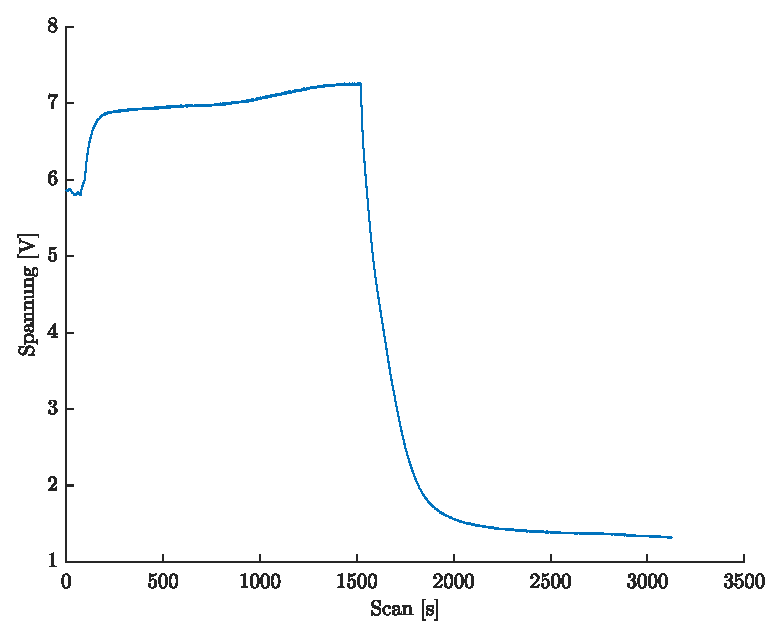
\includegraphics[width=\textwidth]{../DATA/Messreihe_Feuchtekalibration.eps}
	\caption[Kalibrationsmessung]{Kalibrationsmessung anhand zweier Salzlösungen. Zum Zeitpunkt t=\SI{1500}{\second} wurde der Sensor von der NaCl-Lösung über die LiCl-Lösung überführt.}
	\label{fig:cal}
\end{figure}

Aus Abbildung \ref{fig:cal} geht hervor, dass die Spannungen nicht konstant gemessen wurden. Für eine genauere Kalibration ist eine längere Verweilzeit über den Salzlösungen nötig. Prinzipiell eignen sich die gewählten Messpunkte gut, da die Luftfeuchte über den verwendeten Lösungen nahezu temperaturunabhängig ist. Zur genaueren Kalibration müssten jedoch weitere Messpunkte bestimmt werden, da der Sensor nicht zwangsweise ein lineares Verhalten aufweist, welches für die Kalibrierung angenommen wurde. Aus den beiden Kalibrierpunkten und Einsetzen der Umgebungsfeuchte ergibt sich folgende Kalibriergleichung:

\begin{equation}
	\label{eq:cal}
	\varphi(U)=10,65*\SI{5,979}{\volt}-2,167=\SI{61,5}{\percent}
\end{equation}

Zur Umrechnung der absoluten Feuchte wird der temperaturabhängige Sättigungspartialdampfdruck des Wassers näherungsweise nach Gleichung \ref{eq:pds} bestimmt und in Gleichung \ref{eq:x} eingesetzt. 

\begin{multline}
	\label{eq:pds}
	p_{\text{D,S}}(\SI{24}{\celsius}) = 611*exp(-1,91275*10^{-4}+7,258*10^{-2}*\SI{24}{\celsius}-2,939*10^{-4}\\*(\SI{24}{\celsius})^2 +9,841*10^{-7}*(\SI{24}{\celsius})^3-1,92*10^{-9}*(\SI{24}{\celsius})^4)=\SI{2982,47}{\pascal}
\end{multline}

\begin{equation}
	\label{eq:x}
	x=0,622*\frac{p_{\text{D,S}}*\varphi}{p-p_{\text{D}}}=\frac{\SI{2982,47}{\pascal}*\SI{61,5}{\percent}}{\SI{100000}{\pascal}-\SI{1834,52}{\pascal}}=\SI{0,0116}{\kilogram\per\kilogram}
\end{equation}

		
\subsection{Niederschlag}
Zur Berechnung des simulierten Niederschlags wurden die Messdauer und Impulszahl ermittelt. Das Volumen einer Kippwaage ist mit \SI{2}{\cubic\centi\meter} angegeben. Somit entspricht das Testvolumen von einem Liter in der Theorie 500 Impulsen. Zum Vergleich wurde das Waagenvolumen ebenfalls aus dem Kehrwert der Impulszahl berechnet (Auswertung s. folgende Tabelle.)

 \begin{table}
 	\centering
 	\caption{Messdaten der Kippwaage zur Ermittlung der Niederschlagsmengen.}
 	\begin{tabular}{cccc}
 		\label{tab:rain}
 		\textbf{Messung} & \textbf{Impulszahl} n & \textbf{Messdauer} s & \textbf{$V$ pro Impuls} \si{\cubic\centi\meter}\\
 		\hline
 		1 & 166 & 168  & 6,0\\
 		2 & 200 & 105  & 5,0\\
 		3 & 153 & 171  & 6,5\\
 		Mittel & 173 & 148  & 5,9
 	\end{tabular}
 \end{table}

Das Messergebnis ist in erster Linie vom Impulsübertrag auf die Wippe abhängig. Bei geringerem Zufluss wird Wippe durch die Gewichtskraft entleert, bei starkem Niederschlag durch die Strömung des Wassers frühzeitig gekippt. Das theoretische Volumen weicht bei Messung 2 am meisten vom tatsächlichen ab. Die Messmethode ist daher tendenziell für die Messung leichter Regenschauer geeignet. Bei Starkregen versagt sie. 
Die normierte Niederschlagshöhe ergibt sich entsprechend Gleichung \ref{eq:rain2} aus dem Quotienten der Niederschlagsmenge und Trichterfläche (Annahme laut Skript \SI{0,02}{\square\meter}):

\begin{equation}
	\label{eq:rain2}
	h = \frac{V}{A} = \frac{\SI{0,001}{\cubic\meter}}{\SI{0,02}{\square\meter}} = \SI{0,05}{\meter} = \SI{50}{\milli\meter}
\end{equation}

\subsection{Windmessung}
Eine sinnvolle Messung der Luftströmung war aufgrund der ungünstigen Position der Messstation nicht möglich. Daher wird auch bei diesem Versuchsteil auf einen bereitgestellten Datensatz zurückgegriffen. Zunächst ist die Aufnahme der Windrichtung in Abbildung \ref{fig:winddir} gezeigt. Ohne weitere Datenaufarbeitung ist der Datensatz kaum interpretierbar. Die statistische Verteilung ist in Abbildung \ref{fig:winddirCN} dargestellt.
\begin{figure}[H]
	\centering
	\begin{minipage}[t]{0.4\textwidth}
		\centering
		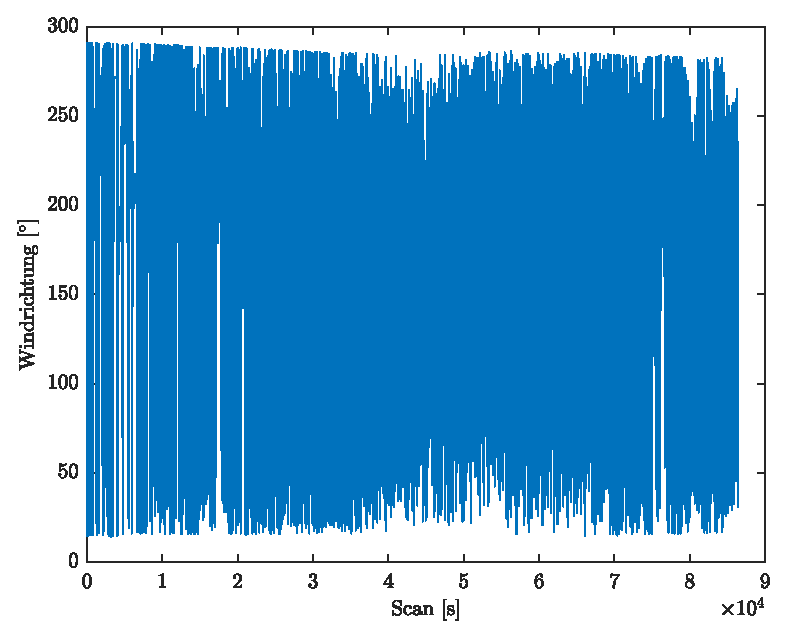
\includegraphics[width=\textwidth]{../DATA/Windrichtung.eps}
		\caption[Windrichtung]{Windrichtung.}
		\label{fig:winddir}
	\end{minipage}
	\hfill
	\begin{minipage}[t]{0.4\textwidth}
		\centering
		\centering
		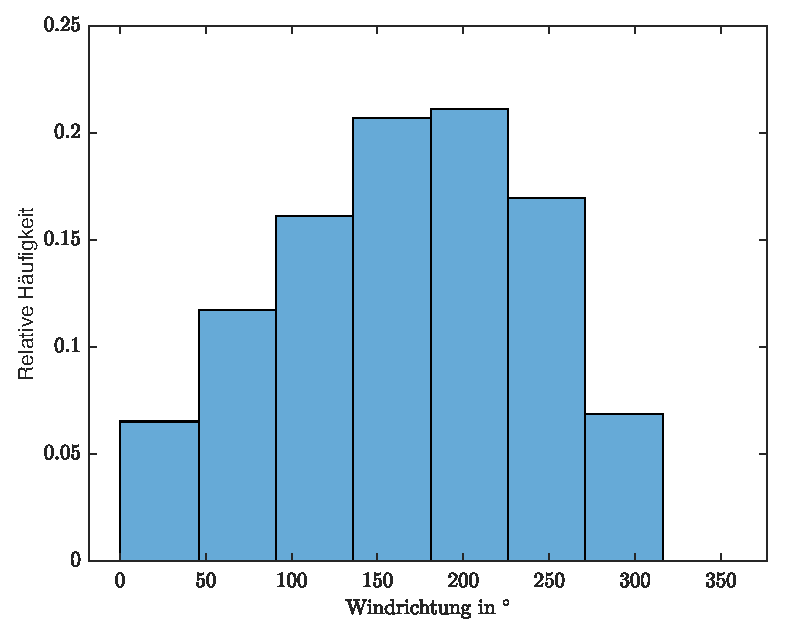
\includegraphics[width=\textwidth]{../DATA/WinddirCN.eps}
		\caption[Windrichtung Verteilung]{Windrichtung Verteilung.}
		\label{fig:winddirCN}
	\end{minipage}
\end{figure}

Etwa 40\,\% der Zeit wehte der Wind aus Richtung SSO bis SSW. Weitere 30\,\% der Zeit aus SWS bzw. OSO zu gleichen Teilen. Die verbleibenden Anteile fallen stärker auf die nordöstliche Richtung als Nordwest. Aus Richtung NNW wehte der Wind nie. Die Windgeschwindigkeit kann bereits anhand der Rohdaten (vgl. Abbildung \ref{fig:windspd}) interpretiert werden. Zu großen Anteilen betrug die Windgeschwindigkeit zwischen 0 und \SI{1}{\meter\per\second}. Zwischenzeitlich wurde eine Spitze mit \SI{5}{\meter\per\second} gemessen. Die Häufigkeitsverteilung (Abbildung \ref{fig:windspdCN}) bestätigt diese Beobachtung. Die Geschwindigkeitsklasse 0 bis \SI{1}{\meter\per\second} ist mit einer statistischen Häufigkeit von 0,8 vertreten, gefolgt von 1 bis \SI{2}{\meter\per\second} mit einer Häufigkeit von 0,1.
\begin{figure}[H]
	\centering
	\begin{minipage}[t]{0.4\textwidth}
	\centering
	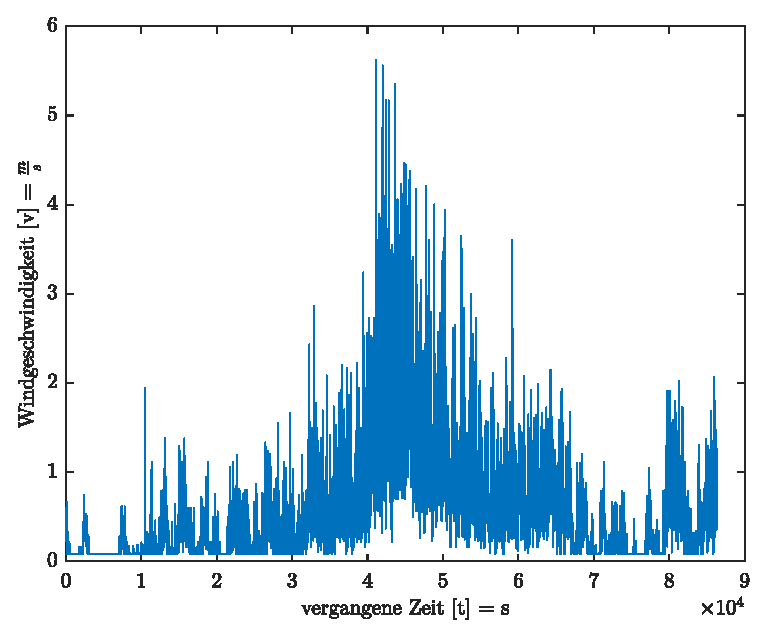
\includegraphics[width=\textwidth]{../DATA/Windgeschwindigkeit.eps}
	\caption[Windgeschwindigkeit]{Windgeschwindigkeit.}
	\label{fig:windspd}
	\end{minipage}
\hfill
	\begin{minipage}[t]{0.4\textwidth}
	\centering
	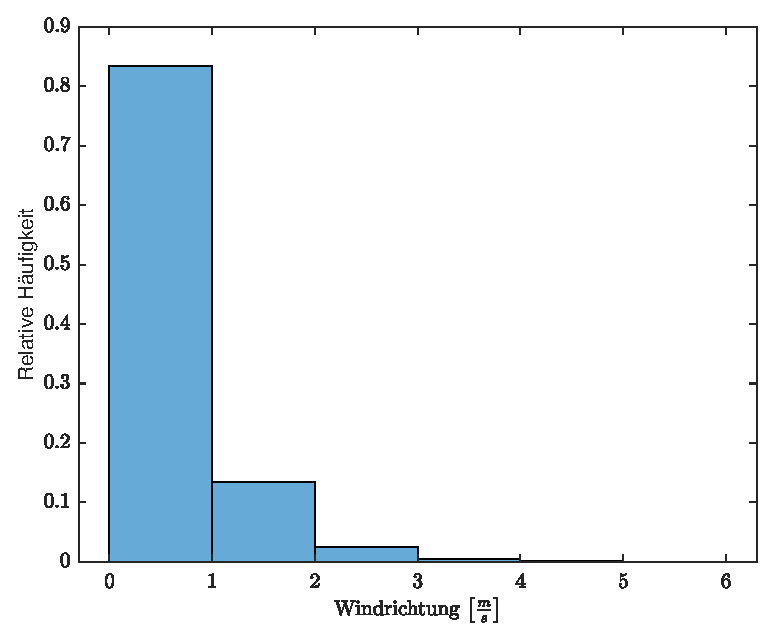
\includegraphics[width=\textwidth]{../DATA/WindspdCN.eps}
	\caption[Windgeschwindigkeit Verteilung]{Geschwindigkeitsverteilung.}
	\label{fig:windspdCN}
	\end{minipage}
\end{figure}
